\documentclass[handout]{beamer}

\usetheme{Siegen}
\usecolortheme{LILA} 


% Im Beamertheme Siegen ist festgelegt:
% 1. Innertheme: Alles was auf der weißen Fläche in der Mitte passiert (Blocks, enumerate,...)
% 2. Outertheme: Alles was in den Kopf und Fußzeilen passiert.
% 3. Colortheme: Alles was mit Farben zu tun hat.

% Variationen
% Mit "\useinnertheme{xxx}", "\useoutertheme{xxx}" und "\usecolortheme{xxx}" können die einzelnen Teile unabhängig voneinander verändert werden.

% 1. Das Innertheme kann natürlich uneingeschränkt verändert werden, ohne vom Corporate design abzuweichen. (Möglichkeiten siehe beameruserguide.pdf) 

% 2. Das Outertheme ist für das Corporate design verantwortlich. Theoretisch muss die Fußzeile nur blau sein, was darin steht ist jedem selbst überlassen. Ich habe hier Referent (Uni) und einen Folienzähler verortet. Wenn das geändert werden soll, muss man direkt in den Quellcode von "beamerouterthemecdSiegen.sty" eingreifen.  

% 3. Colortheme: 
% a) Colortheme "GELB" (Uni-blau und Uni-Sekundärfarbe-gelb/organge) 
%    [default-Einstellung] 
% b) Colortheme "LILA" (Uni-blau und Fakultäts-lila)


\usepackage{graphicx}
\usepackage[utf8]{inputenc}
\usepackage[ngerman]{babel}
\usepackage{amsmath, amssymb, amsfonts, amsthm, dsfont}
\usepackage{tikz}
\usepackage{siunitx}
\usepackage{graphicx}
%\usepackage{pdfpages}

\usepackage{feynmp-auto}
%\usepackage{feynmp}
\DeclareGraphicsRule{*}{mps}{*}{}
\unitlength = 1mm


\hypersetup{pdfborderstyle={/S/U/W 0}} % das brauche ich, damit meine Tex-Version nicht komische Verlinkungen zwischen den Sektions macht -- ihr braucht das vielleicht nicht, aber es schadet auch nicht.


% Folgende Zeilen definieren meine Zitat-Umgebung:
\newcommand{\Untertitel}
  {\begin{flushright}\tiny \rm\textsc{\Quelle}\end{flushright}}

\newenvironment<>{zitat}[1]%
{\begin{beamerboxesrounded}[upper=white, lower=white, shadow=true]{}%
 \newcommand{\Quelle}{#1}}%
{\Untertitel\end{beamerboxesrounded}}



\title{Email Crypto }
\subtitle{Jetzt geht es ans Eingemachte!}
%\subtitle{Crypto Workshop}
\author[]{Benedikt Schmitz}
\institute[Uni Siegen]{Crypto-Initiative \\ Universität Siegen}
\date{\today}

\begin{document}
\begin{frame}

  \maketitle  

\end{frame}

\begin{frame}{}
  
  \tableofcontents%[pausesections]

\end{frame}

\section{Crypto!}
\subsection{Let's get started!}
\begin{frame}{Before}
    Windows: 
    \begin{enumerate} 
        \item Download GPG4Win \url{www.gpg4win.org}\pause
        \item Install GPG4Win \pause
        \item Install Enigmail
    \end{enumerate}\pause
    Linux:
    \begin{enumerate}
    \item Install Enigmail
    \end{enumerate}
\end{frame}
\begin{frame}{}
    \begin{center}
        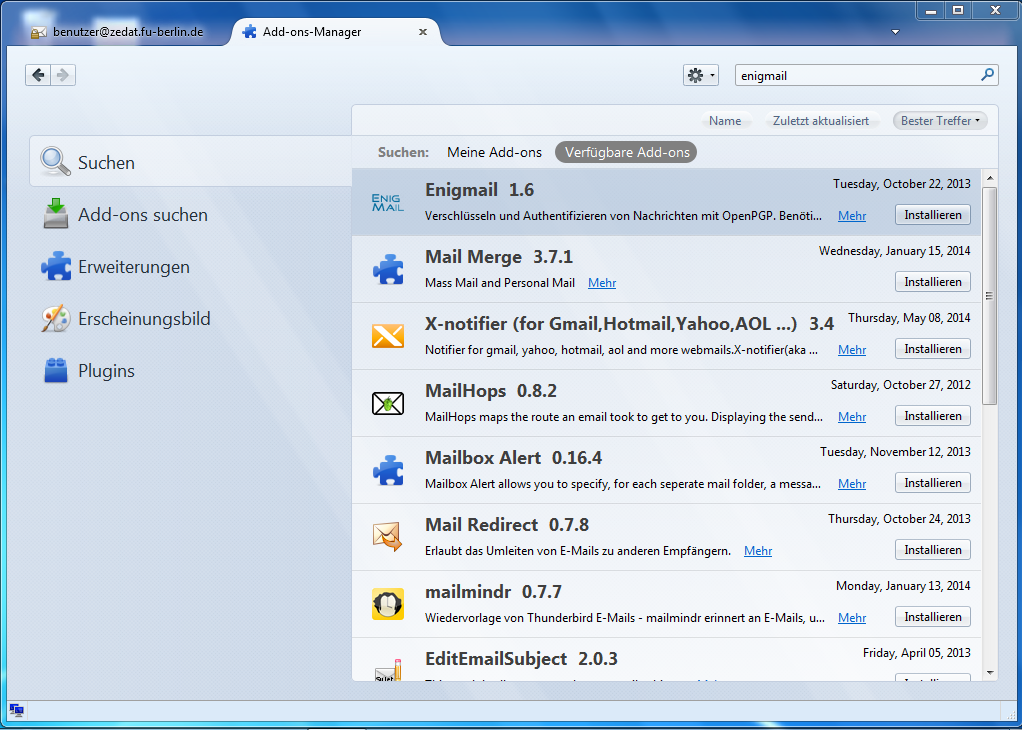
\includegraphics[width=0.9\textwidth]{Bilder/enigmail.png}
    \end{center}
\end{frame}

\subsection{Exkurs: Cryptosysteme}

%\begin{frame}{}
%	\begin{block}{Verschlüsselungsverfahren}
%		\begin{itemize}
%			\item Symmetrisches Cryptosystem  
%			\item Asymmetrisches Cryptosystem
%			\item Vorteile/Nachteile
%		\end{itemize}
%	\end{block}
%\end{frame}
\begin{frame}{Symmetrisches Cryptosystem}
	\begin{block}{}
		\begin{center}
			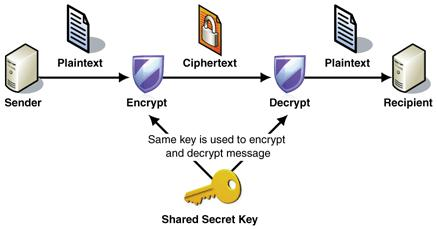
\includegraphics[scale=0.6]{Bilder/PGP1.jpg}
		\end{center}%\footnote{Grafik auf deutsch!}
%		\begin{itemize}
%			\item Es existiert nur 1 Schlüssel. 
%			\item Algorithmen: 
%				\begin{itemize}
%					\item[PGP]	TripleDES, IDEA, CAST5, Blowfish
%					\item[S/MIME] TripleDES, DES, RC2
%				\end{itemize}					
%		\end{itemize}
	\end{block}
\end{frame}
\begin{frame}{Asymmetrisches Cryptosystem}
	\begin{block}{}
		\begin{center}
			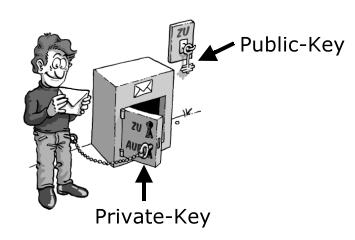
\includegraphics[scale=0.6]{Bilder/PGP2.jpg}
		\end{center}
%		\begin{itemize}
%			\item Es existieren 2 Schlüssel. Private und Public
%			\item Algorithmen: 
%				\begin{itemize}
%					\item[PGP]	RSA, DSA (Signatur)
%					\item[S/MIME] RSA
%				\end{itemize}					
%		\end{itemize}
	\end{block}
\end{frame}

\begin{frame}{Unterschiede}
	\begin{block}{}
		\begin{center}
			\begin{tabular}{|c||c|}\hline
				Symmetrisch & Asymmetrisch \\ \hline \hline
				ein gemeinsamer Schlüssel & 2 Schlüsselpaare (4 Schlüssel) \\ \hline
				Sichere Übertragung nötig & Keine sichere Übertragung nötig \\ \hline
				keine Signatur möglich & Signatur möglich \\ \hline
				schnell & nicht so schnell \\\hline
			\end{tabular}
		\end{center}%\footnote{Formulierung überprüfen!}
		%\begin{itemize}
		%	\item Allgemein: Asymmetrisch potenter aber nicht so schnell.
		%	\item Symmetrisches System kann einen sicheren Austausch bekommen $\to$ Diffie-Hellmann 
		%\end{itemize}
	\end{block}
\end{frame}

\subsection{How to PGP}

\begin{frame}{Reboot}
    \begin{center}
        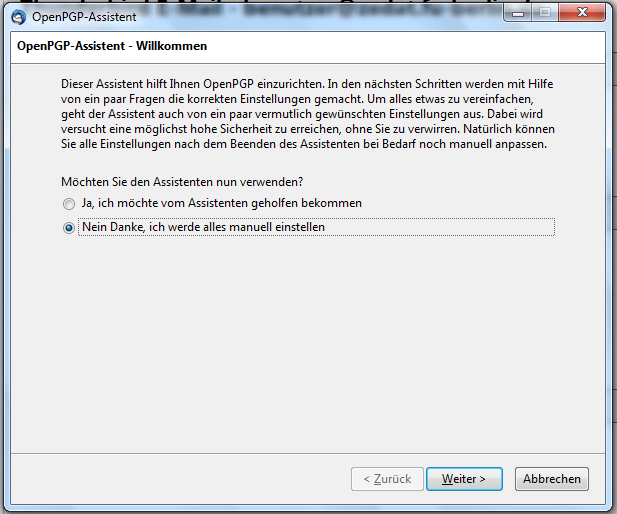
\includegraphics[width=\textwidth]{Bilder/enigmail1.png}
    \end{center}
\end{frame}

\begin{frame}{}
    \begin{center}
        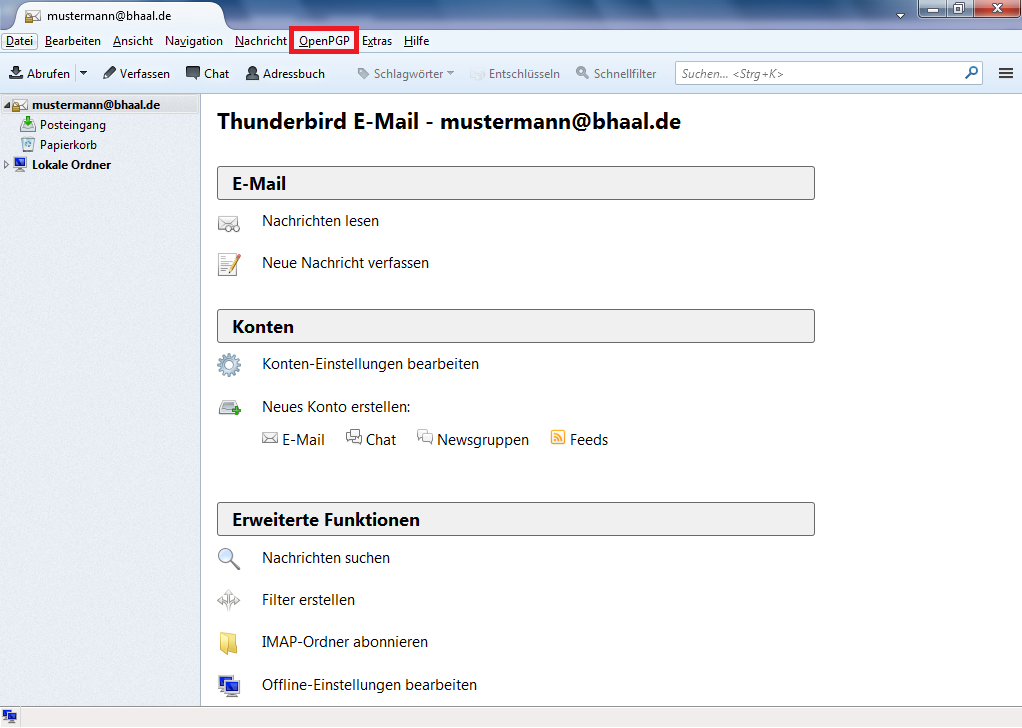
\includegraphics[width=\textwidth]{Bilder/enigmail2.png}
    \end{center}
\end{frame}
\begin{frame}{}
    \begin{center}
        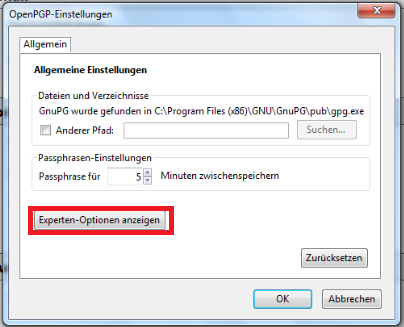
\includegraphics[width=\textwidth]{Bilder/enigmail3.png}
    \end{center}
\end{frame}

\subsection*{Passphrase}
\begin{frame}{Passphrase}
    \begin{center}
        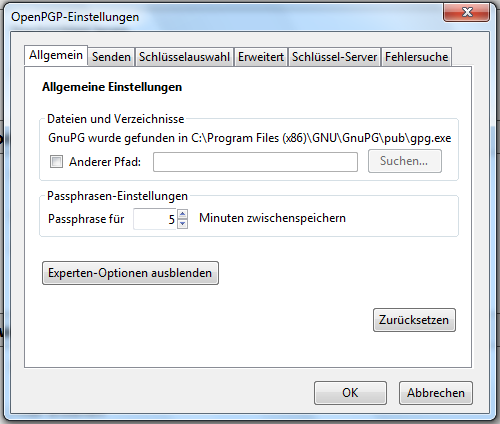
\includegraphics[width=\textwidth]{Bilder/enigmail4.png}
    \end{center}
\end{frame}
\begin{frame}{Was ist die Passphrase?}
    \begin{center}
        \begin{itemize}
        \item Passphrase entsperrt privaten Schlüssel. \pause
        \item[$\Rightarrow$] Bei jedem Senden und Entschlüsseln eingeben! \pause
        \item[$\Rightarrow$] Also um Zeit zu sparen: Zeit setzen, für die der Schlüssel gültig bleibt. \pause %FIXME der Schlüssel bleibt länger gültig, eigentlich merkt er sich nur das Passwort für die Dauer im Cache
        \item Gute Zeit: Zwischen 1 und 5 Minuten
        \end{itemize}
    \end{center}
\end{frame}

\begin{frame}{}
    \begin{center}
        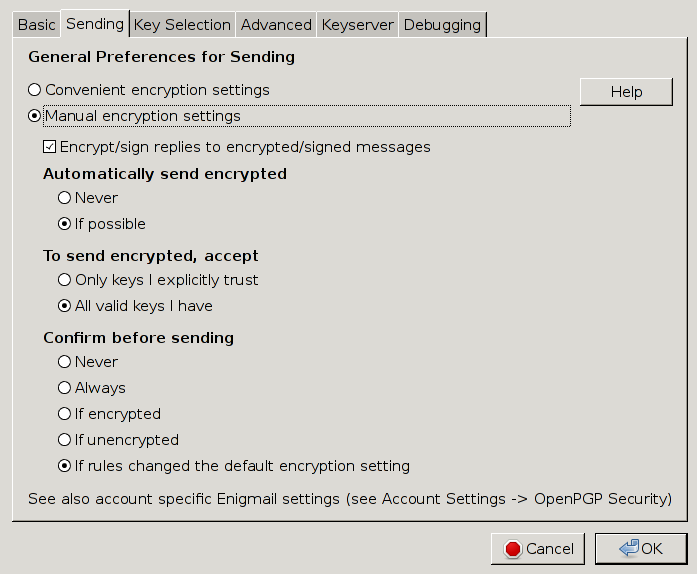
\includegraphics[scale=0.4]{Bilder/enigmail5.png}
    \end{center}
\end{frame}

\begin{frame}{}
    \begin{center}
        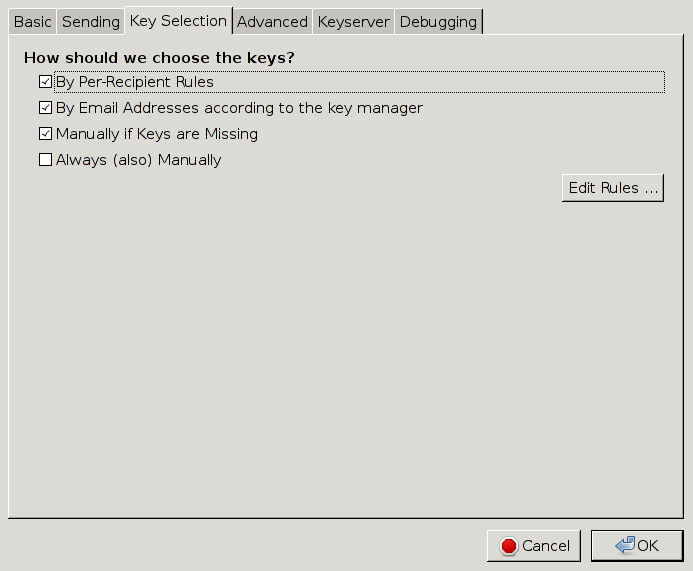
\includegraphics[scale=0.4]{Bilder/enigmail6.png}
    \end{center}
\end{frame}

\begin{frame}{}
    \begin{center}
        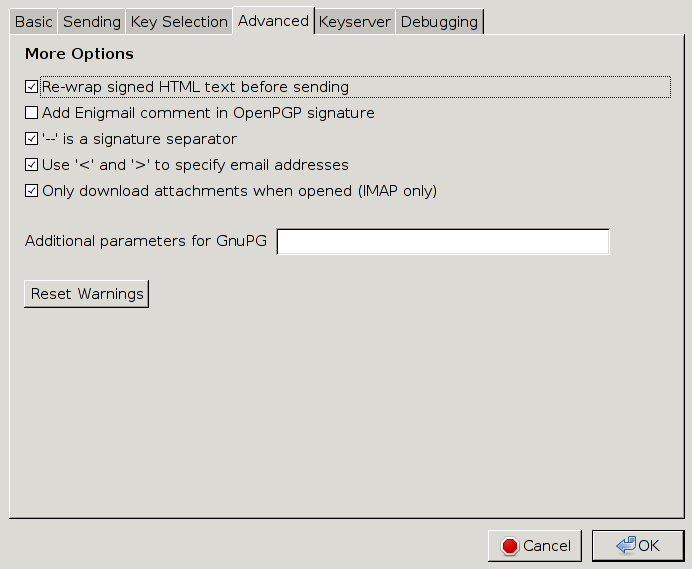
\includegraphics[scale=0.4]{Bilder/enigmail7.png}
    \end{center}
\end{frame}

\subsection{Let's talk about keys baby...}

\begin{frame}{}
	\begin{block}{}
		\begin{itemize}
			\item PGP verwendet asymmetrische Cryptoverfahren  \pause
			\item Public-Key ist öffentlich zugänglich
			\item Mit Public-Key wird verschlüsselt und Signatur geprüft! \pause
			\item Private-Key muss privat und unzugänglich sein
			\item Mit Private-Key wird entschlüsselt und Signatur gesetzt!\pause
		\end{itemize}
	\end{block}
	\begin{block}{Wichtig!}
		\begin{itemize}
			\item Kommunikation ist nötig! Schlüssel müssen verbreitet werden! ($\to$ Schlüssel-Server, Homepage)\pause
			\item Keys \textbf{gehören} zusammen, haben aber keinen offensichtlichen Zusammenhang ($\to$ Faktorisierung/Diskreter Logarithmus)
		\end{itemize} 
	\end{block}
\end{frame}

\begin{frame}{}
    \begin{center}
        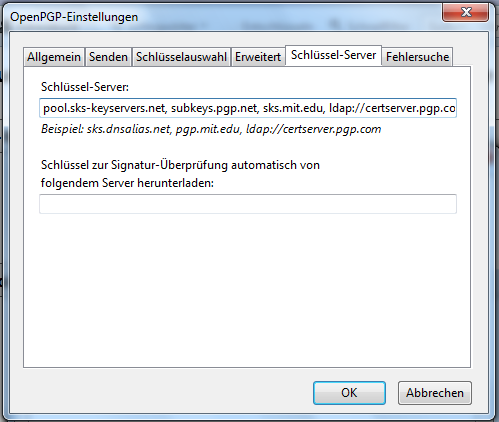
\includegraphics[scale=0.6]{Bilder/enigmail8.png}
    \end{center}
\end{frame}

\subsection{...lets talk about how...}

\begin{frame}{}
    \begin{center}
        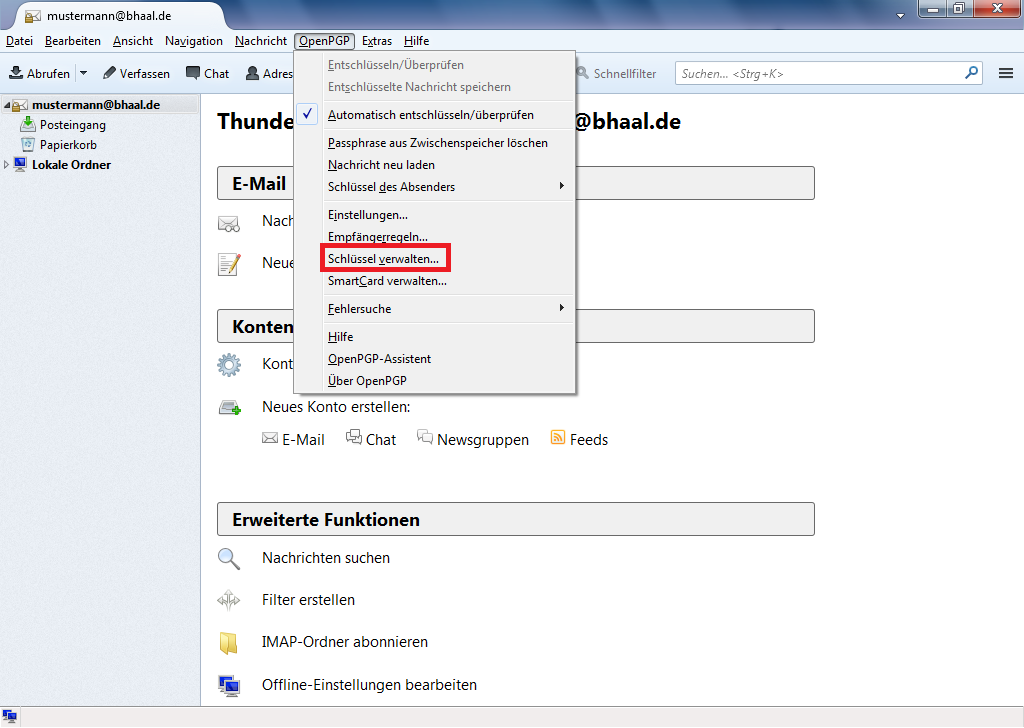
\includegraphics[scale=0.4]{Bilder/enigmail9.png}
    \end{center}
\end{frame}
\begin{frame}{}
    \begin{center}
        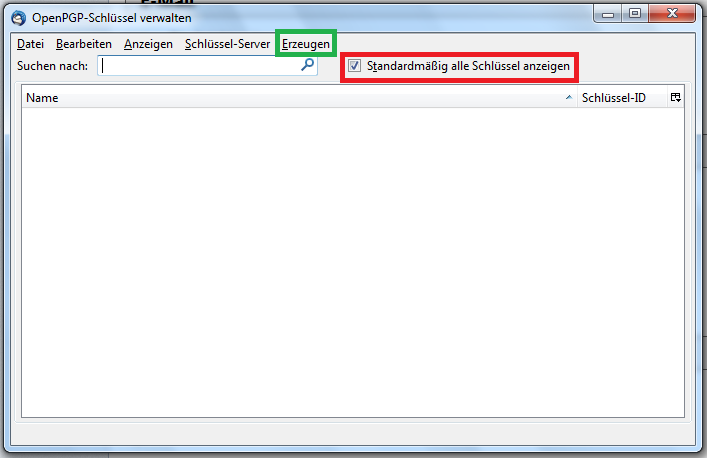
\includegraphics[scale=0.6]{Bilder/enigmail10.png}
    \end{center}
\end{frame}

\begin{frame}{}
    \begin{center}
        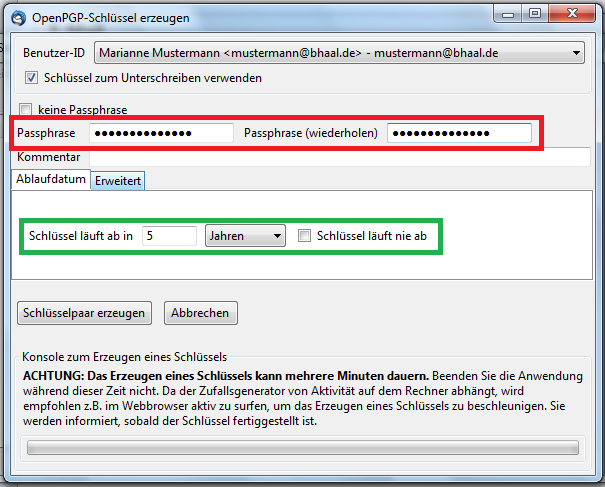
\includegraphics[scale=0.6]{Bilder/enigmail11.png}
    \end{center}
\end{frame}

\begin{frame}{}
    \begin{center}
        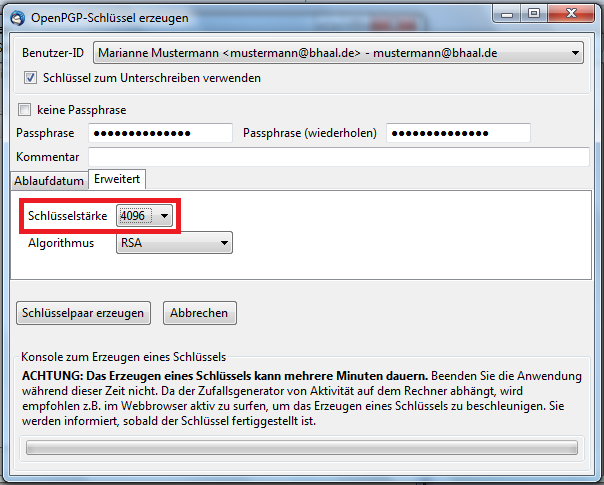
\includegraphics[scale=0.6]{Bilder/enigmail12.png}
    \end{center}
\end{frame}

\begin{frame}{}
    \begin{center}
        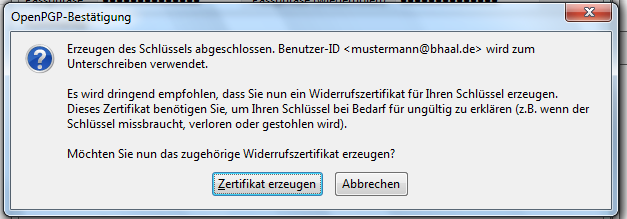
\includegraphics[scale=0.6]{Bilder/enigmail13.png}
    \end{center}
\end{frame}

\begin{frame}{}
    \begin{center}
        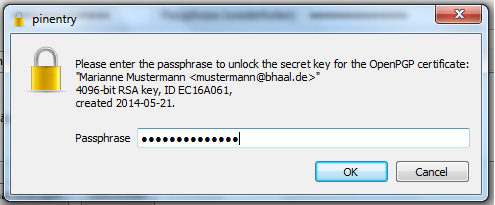
\includegraphics[scale=0.6]{Bilder/enigmail14.png}\\
        
\includegraphics[scale=0.6]{Bilder/enigmail15.png}
    \end{center}
\end{frame}

\begin{frame}{}
    \begin{center}
        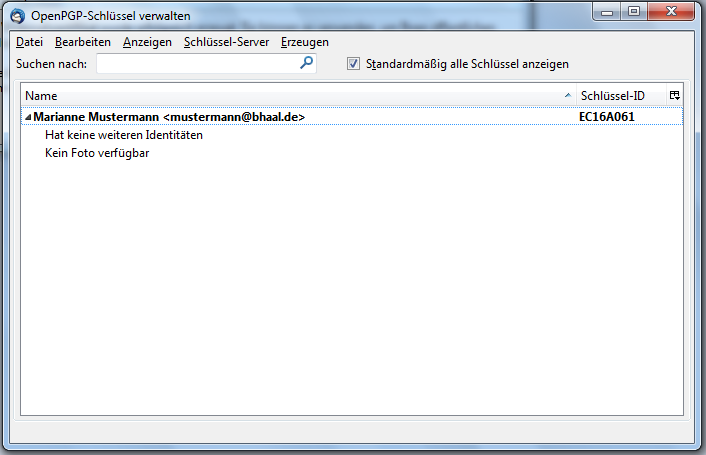
\includegraphics[scale=0.6]{Bilder/enigmail16.png}
    \end{center}
\end{frame}
%\subsection{Authentifikation}

%\begin{frame}{}
%	\begin{block}{Wie authentifizieren wir unsere Schlüssel?}
%		\begin{center}
%			\begin{tabular}{l||l}
%				PGP: Web of Trust & S/MIME: TrustCenter \\ \hline\hline
%				a) User certify the Keys  & Only Institutions certify\\
%				b) Institution certify Keys & \\
%				certified/signed keys published & \\
%				external certification not needed& \\ 
%			\end{tabular}\pause
%		\end{center}
%	\end{block}
%	\begin{block}{Vertrauensniveau:}
%		\begin{enumerate}
%			\item Verifizierung nur per mail: unsicher \pause
%			\item Verifizierung mit genauer Prüfung: Amtliches Papier \pause
%           \item Extrem genaue Prüfung: persönliche Authentifikation
%		\end{enumerate}
%	\end{block}
%\end{frame}

\section{Wars das?}

    \begin{frame}{}
        \begin{center}
            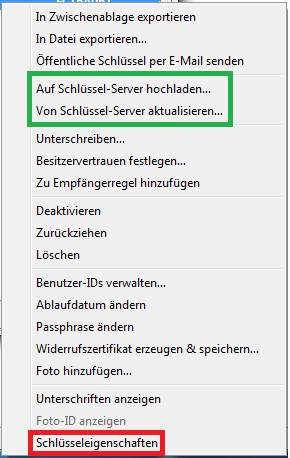
\includegraphics[scale=0.5]{Bilder/enigmail17.png}
        \end{center}
    \end{frame}
    
    \begin{frame}{}
        \begin{center}
            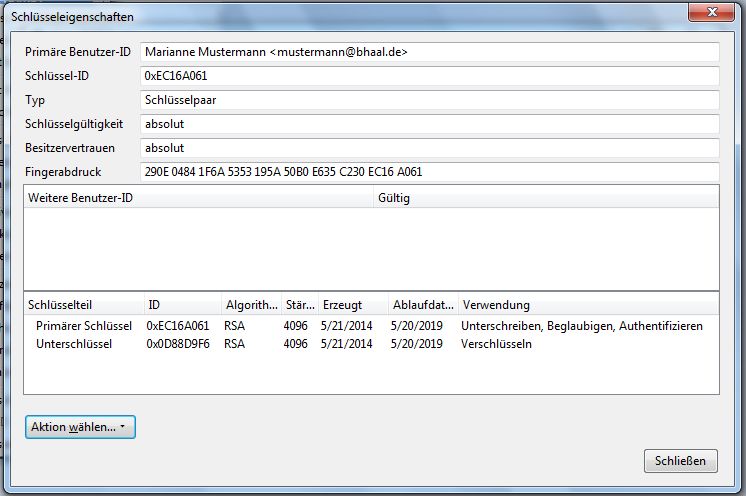
\includegraphics[scale=0.5]{Bilder/enigmail18.png}
        \end{center}
    \end{frame}


\subsection{Schlüsselgültigkeit}
    \begin{frame}{Schlüsselgültigkeit}
        \begin{block}{Wie sehr vertraust du dem Schlüssel?}
            \begin{itemize}
            \item Gar nicht $\rightarrow$ unbekannt
            \item Falls doch $\rightarrow$ eingestellter Wert
            \item Dein Schlüssel $\rightarrow$ absolut
            \end{itemize}
        \end{block} \pause
        \begin{center}
            Vertrauen wird über Signaturen eingestellt. \\
            Du unterschreibst den Schlüssel ($\to$ Praxis)
        \end{center}
    \end{frame}

\subsection{Benutzervertrauen}

    \begin{frame}{Benutzervertrauen}
        \begin{block}{PGP}
            \begin{itemize}
            \item lokale Größe
            \item klassifiziert das Vertrauen, dass jemand korrekt andere Signaturen unterschreibt
            \item variiert einen Zweig im Web of Trust
            \end{itemize}
        \end{block}
        \begin{block}{S/MIME}
            \begin{itemize}
            \item Existiert hier nicht
            \item Alle User durch Trust Center authentifiziert.
            \item Trust Center kompromittiert?
            \end{itemize}
        \end{block}
    \end{frame}
%\subsection{CIA Modell}
%
%\begin{frame}{}
%	\begin{block}{Integrität}
%		\begin{itemize}
%			\item Signature identifies the sender
%		\end{itemize}
%	\end{block}
%\end{frame}

%\begin{frame}{}
%	\begin{block}{Confidentiality}
		
%	\end{block}
%\end{frame}
%
%
%
%\section{Fazit}
%    \begin{frame}{Fazit}
%        Grund-Funktionen und Sicherheit ist bei beiden gleich gut!
%        \begin{minipage}{0.49\textwidth}
%            \begin{block}{PGP}
 %               \begin{itemize}
%                \item kein externes Zertifikat
%                \item extra Addon/Programm
%                \end{itemize}
%            \end{block}
%        \end{minipage}%
%        \begin{minipage}{0.49\textwidth}
%            \begin{block}{S/MIME}
%                \begin{itemize}
%                \item benötigt Zertifikat (kann teuer werden)
%                \item kein extra Addon/Programm
%                \end{itemize}
%            \end{block}
%        \end{minipage}
%    \end{frame}
    
\end{document}
